\chapter{Simulating Hagen Poiseuille flow}
\thispagestyle{empty}
\label{sec:chap9}
\newcommand{\LocCHninefig}{\Origin/CHAPTERS/chap9/figures}

\section{What is Hagen Poiseuille Law}

In nonideal Fluid Dynamics Hagen Poiseuille flow or Poiseuille law is a law which gives presure drop in a fluid flowing through a long cylindrical pipe.This law was experimentally derived independently by Gotthilf Heinrich Ludwig Hagen in 1839 and Jean Leonard Marie Poiseuille in 1838, and published by Poiseuille in 1840 and 1846. The assumptions of the equation are that the fluid is incompressible, Newtonian the flow is laminar through a pipe of constant circular cross-section that is substantially longer than its diameter and there is no acceleration of fluid in the pipe. For velocities and pipe diameters above a threshold, actual fluid flow is not laminar but turbulent, leading to larger pressure drops than calculated by the Hagen–Poiseuille equation.

\section{Problem Specification}

\begin{figure}[h]  
\centering
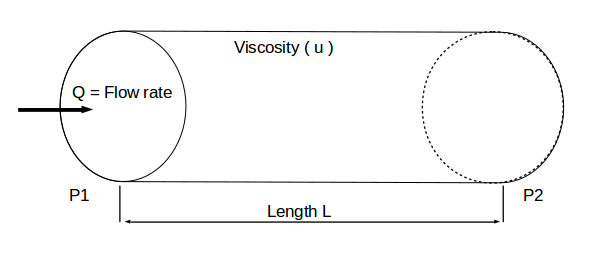
\includegraphics[scale=0.4]{\LocCHninefig/pipe.png}
\caption{Flow through a pipe}
\label{pipe}
\end{figure}

To simulate Hagen Poiseulle flow we consider a pipe of length 0.3m, diameter of 0.01m and fluid medium as water having a dynamic viscosity of $10^{-3}$. The pressure difference in along the pipe is taken as 20 Pascals.\newline

\flushleft Standard governing equations for Pressure drop in the pipe, Fig \ref{pipe} is given as follows, 

\begin{equation}
\nabla p = \frac{32 \mu_avg L }{D^2}
\end{equation}

\flushleft where $\nabla p$ is the pressure loss in the pipe, $\it{L}$ is the length of the pipe, $\mu$ is the dynamic viscosity, $\it{Q}$ is the volumetric flow rate, $\it{r}$ is the radius of the pipe.These parameters have been chosen to get a desired Reynolds number of 2080 which is under transient flow regime.\newline

\flushleft The maximum velocity in the pipe is given as,

\begin{equation}
U_max = 2*U_avg
\end{equation}

\flushleft Subsituting the values in equations above we get the value of $U_{max}$ around 0.416 $\frac{m}{s}$

\section{Geometry}

\begin{figure}[h]  
\centering
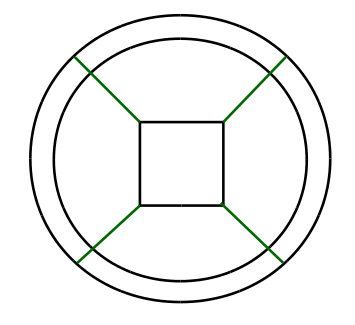
\includegraphics[scale=0.4]{\LocCHninefig/multi.png}
\caption{Multiblock grid}
\label{multi}
\end{figure}

\begin{figure}[h]  
\centering
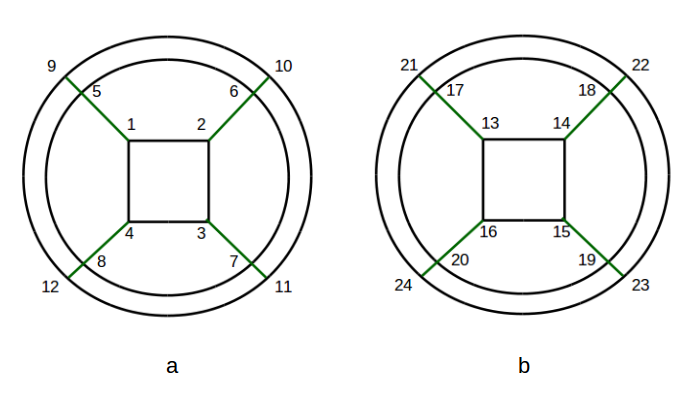
\includegraphics[scale=0.4]{\LocCHninefig/faces.png}
\caption{Back (a) and Front (b) faces for blockMesh}
\label{faces}
\end{figure}

For flow thorugh a pipe we will create a three dimensional pipe using blockMesh. We will use the multiblock meshing, \ref{multi}.This structure gives full control of the mesh grading, using edge meshing, with high-quality elements.Manual creation of multi-block structures can be usually more timeconsuming compared to unstructured meshes.It is seen that the mesh near the walls is required to be finer as compared to the center of the pipe as we can capture the wall shear stresses. In blockMesh we need to define the co-ordinates for each point for front and back faces as shown in the figure, \ref{faces}. For more details on creating a curved geometry in OpenFOAM, refer Chapter number 3. Since it's a 3D problem we will extrude the geometry along the Z direction. The meshing can be kept uniform with 20 cells along X and Y direction and 100 cells along Y direction.

\section{Solver}

Since the flow is still incompressible, viscous and laminar we will choose the solvers from incompressible flow category. We will choose the \textit{icoFoam} solver to solve this problem. \newline

\flushleft Create a folder inside the icoFoam solver directory and name it as pipe. Copy the 0, constant and system folders from the cavity case and paste it inside the newly created pipe folder. 

\subsection{constant}
To start with , make changes inside the blockMeshDict file located inside the polyMesh folder in constant. Edit the blockMeshDict file according to chapter number 3. 
After creating the faces using vertices, we now need to provide boundary names to the faces. This is required since so that we can Identify the different parts of the geometry during visualization and also use appropriate boundary coditions. In this case we have and Inlet, Outlet and walls as the boudnary condition. 

\subsection*{transportProperties}

The \textit{transportPropertis} file can be found inside the constant folder. We set the transport property of the fluid , in this case water and the dynamic visocity of water $\mu$ is taken as $1e^-6$ $\frac{m^2}{s}$
 
\subsection{0 (zero)}
Here we need to provide Initial boundary condition for the pipe. The \textit{0} folder contains files for \textit{pressure} and \textit{Velocity}. Appropriate boundary conditions are provided to solve the case.

\subsection*{p}

At Inlet we provide \textit{fixedValue} since we know the constant value at boundary which is 20 Pa. \newline
\flushleft The outlet is also given as \textit{fixedValue} boudnary condition since it is exposed to the atmosphere and taken as 0 Pa.\newline 
\flushleft The walls are given \textit{zeroGradient} boundary condition as the gradient of Pressure ($\nabla p$) is taken as 0. \newline
The dimension in the folder are given in terms of Kinematic pressure i.e dividing pressure with density and given a unit of $\frac{m^2}{s^2}$.

\subsection*{U}

Inlet boundary condition used for this case we will be \textit{pressureInletVelocity} boundary conditon. It is used when p is known at inlet, U is evaluated from the flux, normal to the patch. The value at inlet for u,v and w components of velocity can be kept as 0.  \newline
\flushleft Outlet boundary condition is taken as \textit{zeroGradient} as the gradient normal to the face is taken as zero. \newline
\flushleft Walls are given a no slip boundary condition and is given a \textit{zeroGradient} boundary condition with u,v and w components of velocity kept as 0.

\subsection{system}

The \textit{fvSchemes} and \textit{fvSolution} files can be kept default. We will change the time setting for our case. As this is a transient case, we keep the endTime of the solution as 20 sec with a time step ($\nabla t$) of $10^{-3}$. We need to make changes in other part of the file. \newline

\flushleft Once these settings are made we are now ready to run the case. Open a Terminal window and type in the path for the pipe folder in the icoFoam case directory of OpenFOAM. After this execute the commands as given below,

\begin{itemize}
\item blockMesh - This will generate the geometry and also mesh according to the mesh grading provided in the file. 
\item checkMesh - This command will check the validity of a mesh i.e Mesh quality, Skewness, number of cells , etc.
\item icoFoam - Run the solver to complete the simulation. The iterations running will be seen in the terminal window.
\end{itemize}

\section{Vizualization}

\begin{figure}[h]  
\centering
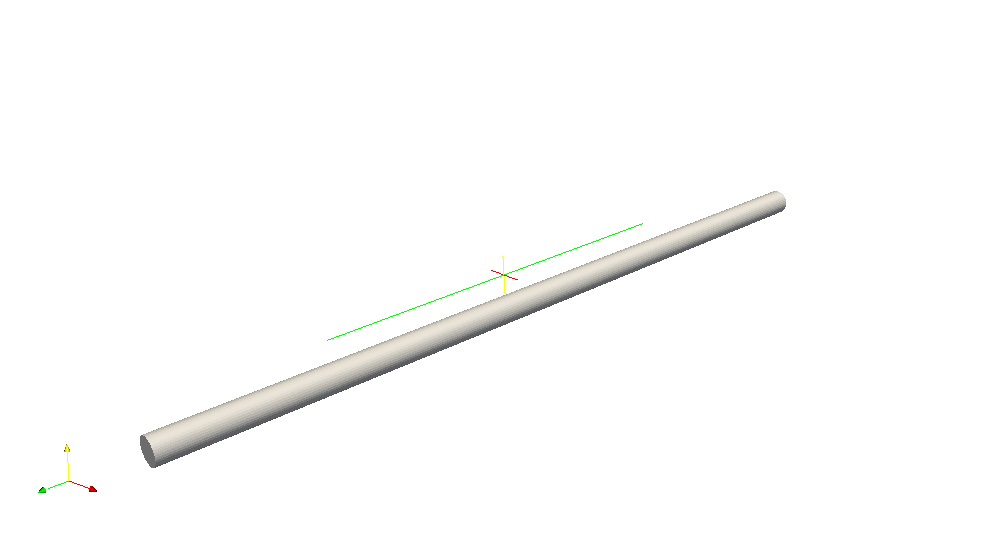
\includegraphics[scale=0.35]{\LocCHninefig/pipe1.png}
\caption{Pipe geometry as seen in Paraview}
\label{pipe_geom}
\end{figure}

\begin{figure}[h]  
\centering
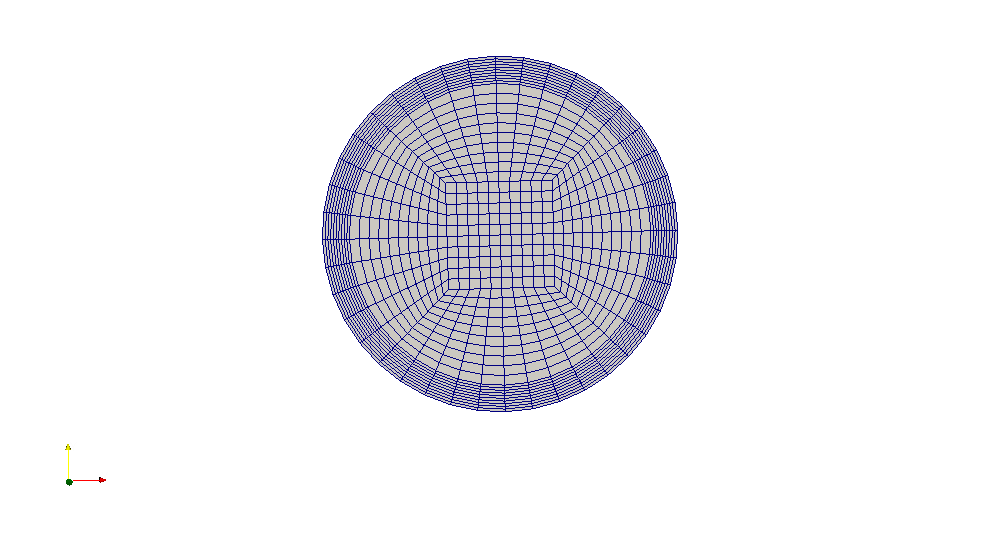
\includegraphics[scale=0.35]{\LocCHninefig/pipe2.png}
\caption{Multiblock mesh}
\label{pipe_mesh}
\end{figure}

\begin{figure}[h]  
\centering
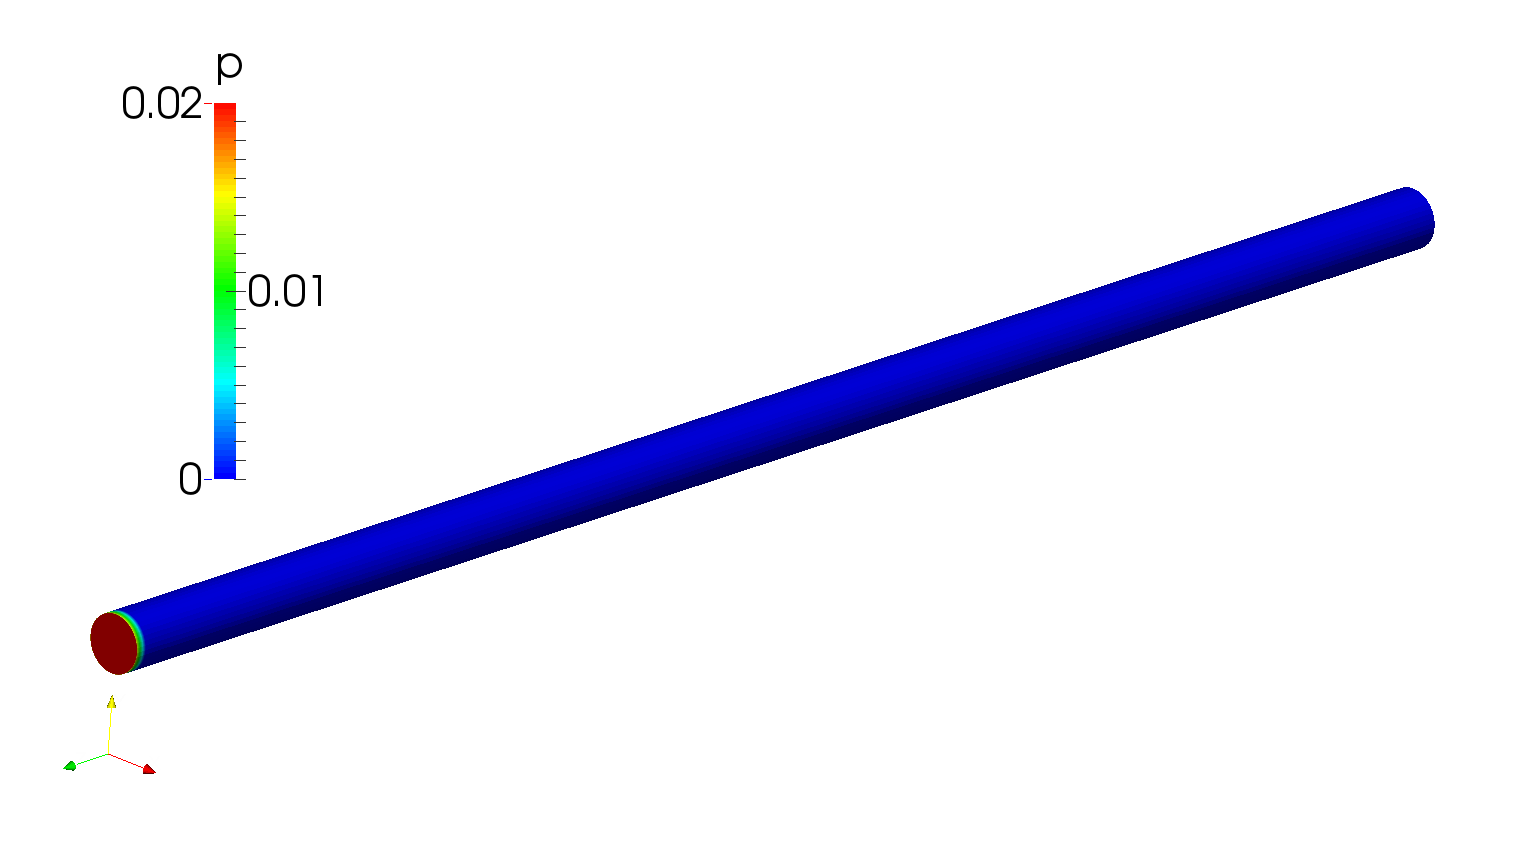
\includegraphics[scale=0.25]{\LocCHninefig/pressure.png}
\caption{Presure on inlet face at time, t = 0 sec}
\label{pipe_pressure}
\end{figure}

\begin{figure}[h]  
\centering
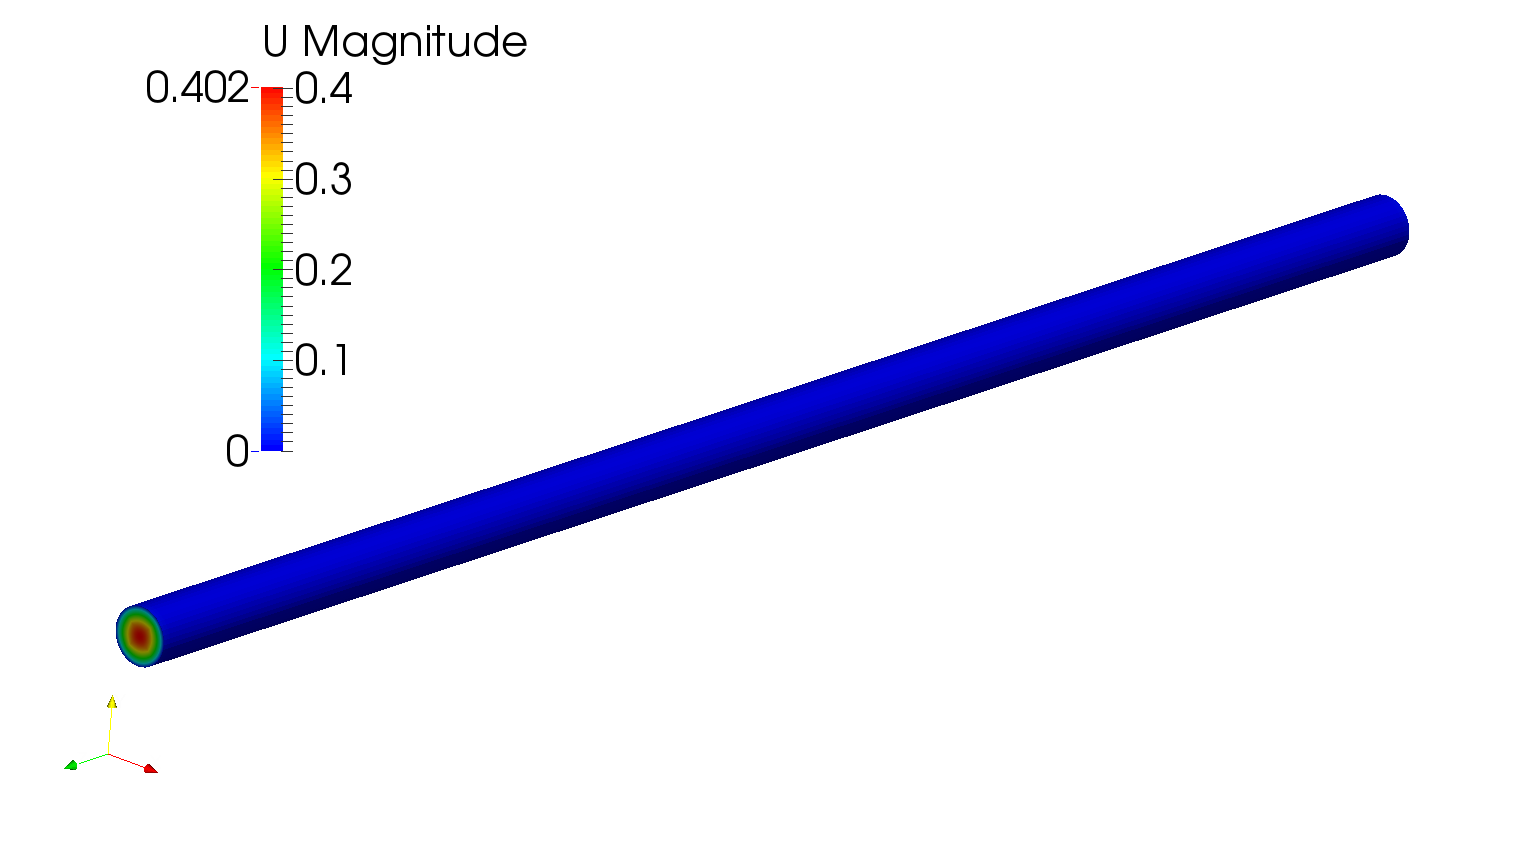
\includegraphics[scale=0.25]{\LocCHninefig/pipe_velocity.png}
\caption{Velocity in the pipe at time , t = 19 sec}
\label{pipe_velocity}
\end{figure}

\begin{figure}[h]  
\centering
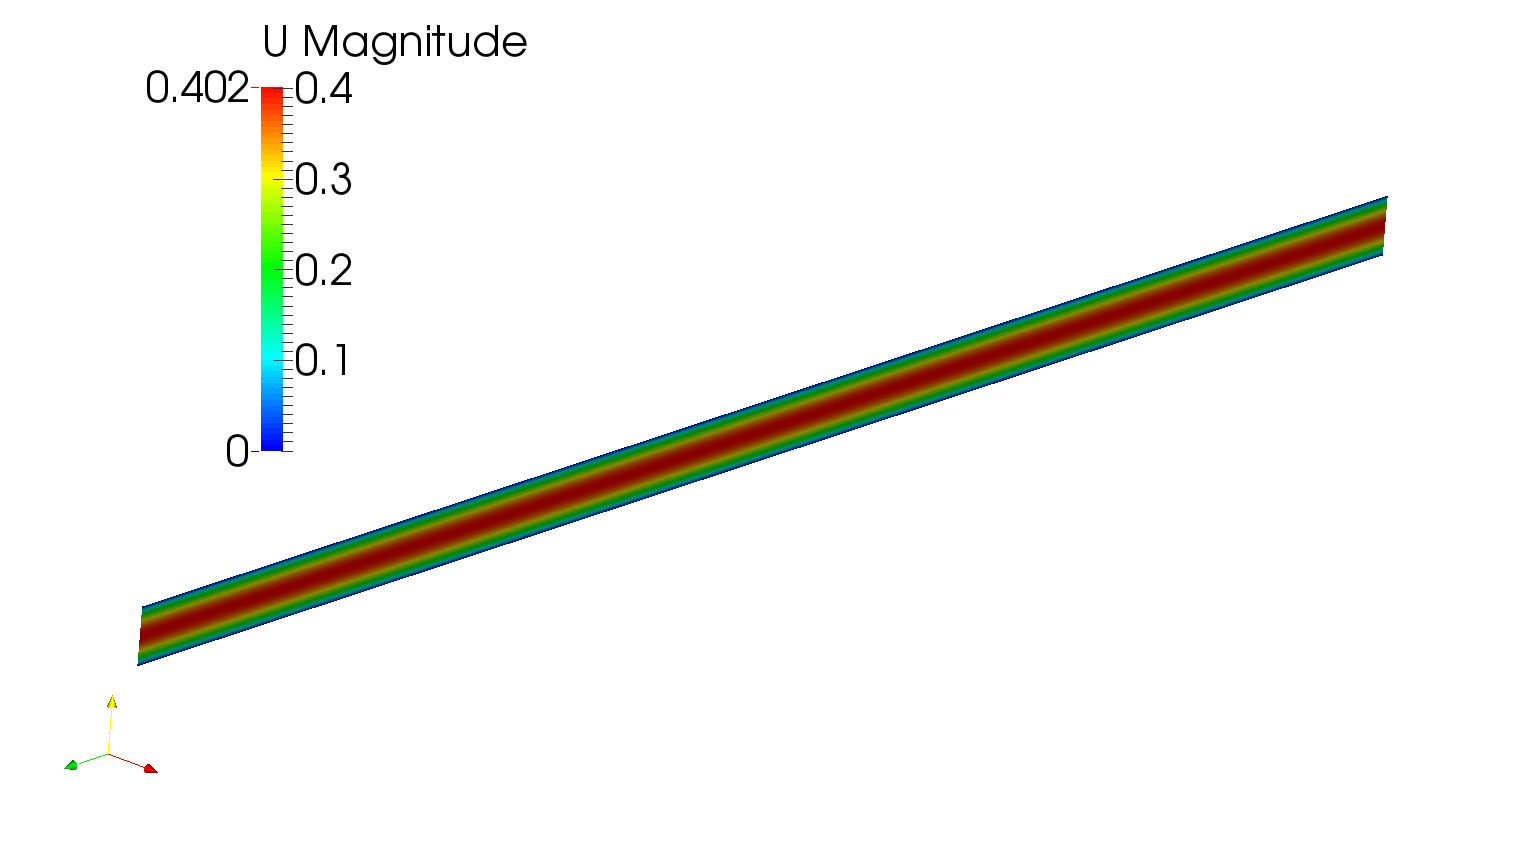
\includegraphics[scale=0.25]{\LocCHninefig/pipe_slice.png}
\caption{Cut section of the pipe showing velocity contour}
\label{pipe_slice}
\end{figure}

\begin{figure}[h]  
\centering
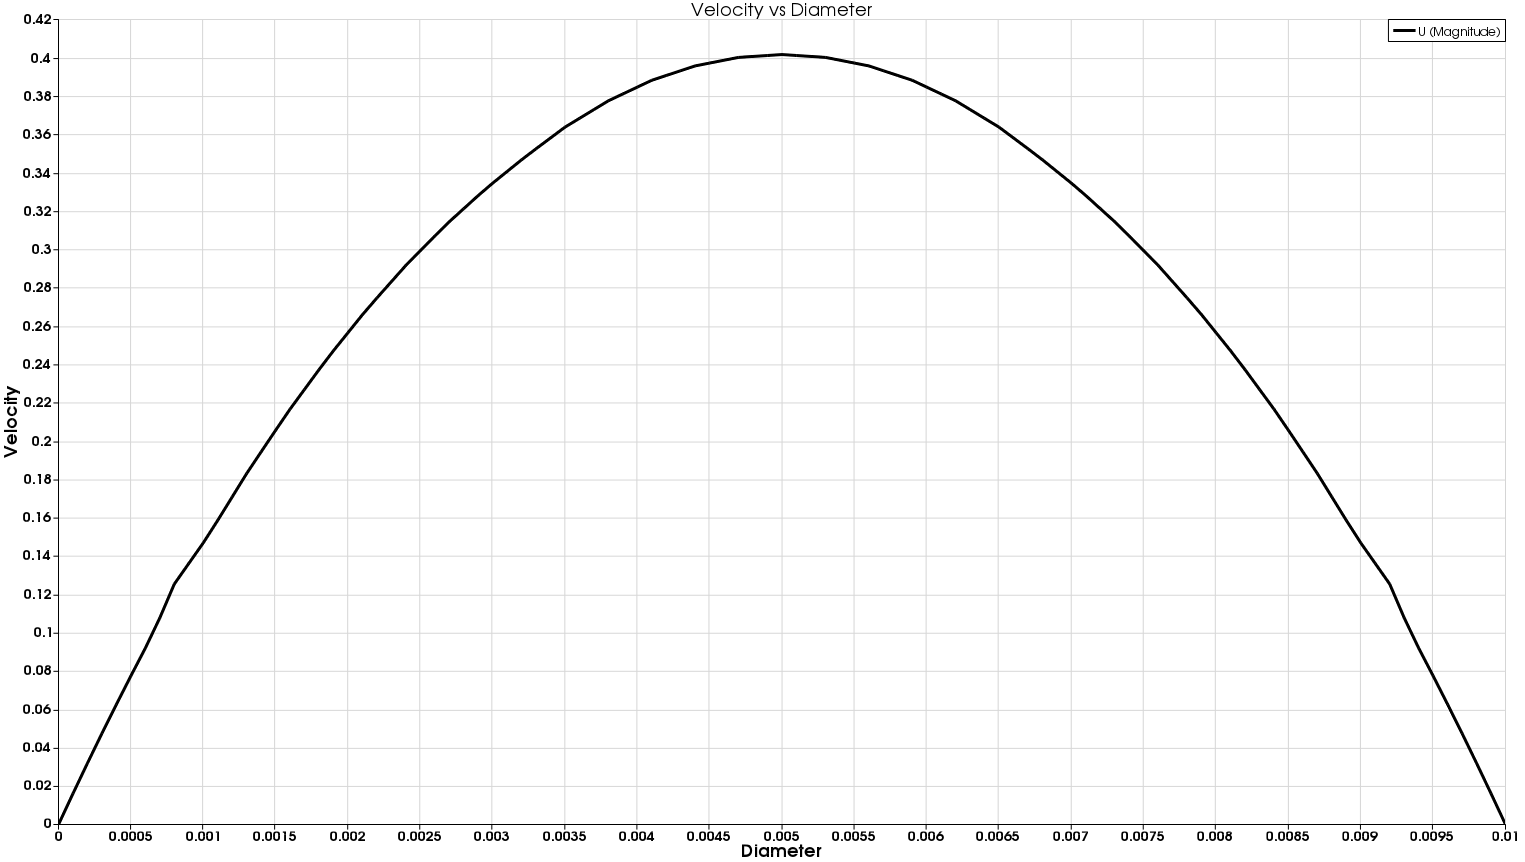
\includegraphics[scale=0.25]{\LocCHninefig/velocity.png}
\caption{Parabolic velocity profile for fully developed flow in the pipe}
\label{pipe_parabolic}
\end{figure}

To visualize the results type \textit{paraFoam} in the terminal and press enter. Click on the Apply button on the left hand Object Inspector menu. This opens up the pipe geometry as seen in Figure \ref{pipe_geom}. Since we have generated a multiblock mesh for this case, to view the same click on the drop down menu below VCR button and change from surface option to Surface with edges. The mesh can now be seen as having a coarse mesh near the center and fine mesh near the wall, Figure \ref{pipe_mesh}.To plot pressure and velocity contours for the pipe, first in the drop down menu change Solid Color to p (pressure). We can see the pressure at inlet of the pipe at time , t = 0 sec, Figure \ref{pipe_pressure}. Click on the play button on the top VCR menu and wait till it reaches the end time of 19 sec. In the drop down menu now change from p (pressure) to U (Velocity) which shows the velocity of the fluid at 19 sec in the color legend as 0.401 $\frac{m}{s}$ as calculated from analytical results. To display the cross section of the pipe on the Top menu in paraview go to \textit{Filter / Alphabetical / Slice }, select as slice along Y axis to get a cut section of the pipe, Figure  \ref{pipe_slice}. The flow developes a parabolic profile once it reaches a sufficient development length. To plot the velocity profile for the flow, go to \textit{Filters / Alphabetical / Plot over Line} and select Y axis and click on Apply. A new window will open showing plots of velocity, pressure. Now scroll down the property pannel and select p ( pressure ) check box. We can see the parabolic velocity profile as seen in the Figure \ref{pipe_parabolic}.

\section{Assignment}

Create a pipe having a diameter of 0.02 m and length of 0.4 m. Pressure at the inlet of the pipe is 100 Pascals and atmospheric at the outlet. Calculate the reynolds number for this flow for a fluid having viscosity of $10^{-6}$ $\frac{m^2}{s}$Carry out simulation for a course grid and a fine grid. Compare both the solution obtained in both the cases. 